\documentclass[a4paper,10pt]{scrartcl}

% IMPORTS
\usepackage{amsfonts}
\usepackage{amsmath}
\usepackage{amssymb}
\usepackage{graphicx}
\usepackage{titlesec}
\usepackage{wrapfig}
\usepackage[ngerman]{babel}
\usepackage[utf8x]{inputenc}
\usepackage{pdfpages}
\usepackage{placeins}
\usepackage{color}
\usepackage{eurosym}
\usepackage{xargs}
\usepackage{xcolor}
\usepackage{subcaption}
\usepackage{hyperref}
\usepackage[margin=2cm]{geometry}
\usepackage[colorinlistoftodos,prependcaption,textsize=tiny]{todonotes}

% CONFIG
\clubpenalty = 9000
\widowpenalty = 9000
\displaywidowpenalty = 9000
\titlespacing\section{0pt}{14pt plus 4pt minus 2pt}{2pt plus 2pt minus 1pt}
\titlespacing\subsection{0pt}{10pt plus 4pt minus 2pt}{2pt plus 2pt minus 1pt}
\setlength{\parindent}{0pt}
\setlength{\parskip}{0.5em}
\setcounter{tocdepth}{3}

\title{Abhängigkeitsanalyse}

% -----------------------------------------------------------------------------
\begin{document}

\maketitle

\tableofcontents
\newpage

\section{Mathematische Grundlagen}
\subsection{Ordnungen}
\subsection{Graphen}

\textbf{Beispielgraph:}

\begin{center}
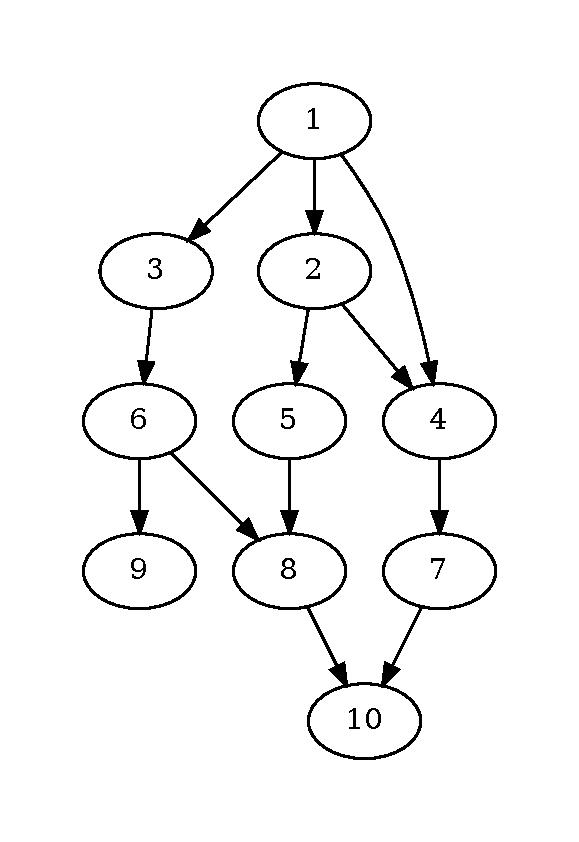
\includegraphics[scale=0.7]{BeispielgraphGraphentheorie.pdf}
\end{center}

\subsubsection{Bestimmung maximaler Ketten}
Von der $1$ an beginnend den Baum aufbauen, Knoten streichen wenn sie durch einen längeren
Pfad erreicht werden können. Tritt ein Knoten mehrfach mit gleicher Distanz zum Anfangsknoten
auf, bleiben beide Ketten bestehen. Sind alle Kanten ausgeschöpft, mit einem anderen Knoten von
vorne beginnen, der noch in keinem Baum aufgetaucht ist (Im Beispiel nicht der Fall).

Hier:
\[1 \rightarrow 3 \rightarrow 6 \rightarrow 9\]
\[1 \rightarrow 3 \rightarrow 6 \rightarrow 8 \rightarrow 10\]
\[1 \rightarrow 2 \rightarrow 5 \rightarrow 8 \rightarrow 10\]
\[1 \rightarrow 2 \rightarrow 4 \rightarrow 7 \rightarrow 10\]

\subsubsection{Bestimmung maximaler Antiketten}
Zunächst die transitive Hülle der Relation bestimmen. Das geschieht im Beispiel idealerweise
bei der 10 beginnend, da Kanten nur von kleineren zu größeren Zahlen existieren. Daraus können
die Antiketten der Länge 2 bestimmt werden. Diese lassen sich immer dann zu längeren Antiketten
verbinden, wenn $\{a,b\}, \{a,c\}, \{b, c\}$ Antiketten sind: Sie bilden zusammen $\{a,b,c\}$.
\textit{Maximale Antiketten} sind die mit der Länge $N$, wenn die längste Antikette $N$
Elemente hat.

Hier:
\[\{1\}, \{2,3\}, \{2,6\}, \{2,9\}, \{3, 4,5\}, \{3, 5, 7\}, \{4, 5, 6\}, \{4,5,9\}, \{4,8,9\},
\{5,6,7\},\{5,7,9\}, \{7,8,9\}, \{9,10\}\]

\subsubsection{Stark und schwach zusammenhängend}
\begin{itemize}
    \item Schwach zusammenhängend: Graph zerfällt nicht in unzusammenhängende Teilgraphen.
    \item Stark zusammenhängend: Jeder Knoten im Graph ist von jedem anderen aus erreichbar.
    \item $n$-fach zusammenhängend: nach dem Löschen von $n−1$ beliebigen Kanten immer noch zusammenhängend
    \item schwache, starke Zusammenhangskomponenten: Teilgraphen, die schwach, stark zusammenhängend sind
    \item azyklische Kondensation: pro starke Zusammenhangskomponente ein Knoten; die “schwachen Kanten” übernehmen
\end{itemize}


\subsection{Matrixalgebra}
\textit{Siehe dumb.pdf Kapitel 3}
\subsection{Fourier-Motzkin}

\section{Abhängigkeitsanalyse im Überblick}
\subsection{Programm-Modell}
\subsubsection{Datentypen:}
\subsubsection{Kontrollstrukturen}
\subsubsection{Iterationen:}
\subsubsection{Ausführungsreihenfolge:}
\subsubsection{Abhängigkeiten:}
\subsubsection{Abhängigkeitsgraphen:}
\subsubsection{Parallelisierung}
\subsection{Abhängigkeiten im allgemeinen}
\subsubsection{Bedingungen (Speicherkonflikt, Existenz, Ordnung, Optimierung, Bernsteinzusatz)}
\subsection{Abhängigkeiten in Schleifenprogrammen}
\subsection{Typen von Abhängigkeiten}
\section{Methoden zur Abhängigkeitsanalyse}
\subsection{Konventionelle Abhängigkeitsanalyse}
\subsection{Polyedermodell}
\subsubsection{Banerjee}
\subsubsection{Feautrier}
    \begin{itemize}
        \item ...
        \item Single-Assignment-Konversion
    \end{itemize}
\subsubsection{Vereinfachte Abhängigkeitsanalyse}
    \begin{itemize}
        \item GCD (einfach und erweitert)
        \item Extreme-Value-Test
    \end{itemize}
\subsubsection{Normalisierung der Array-Indizes}
\section{Eliminieren von Abhängigkeiten}
\section{Ausgewählte Parallelisierungstechniken}



\end{document}

